\section{Охорона праці і навколишнього середовища}
\subsection{Загальні питання охорони праці}
Охорона праці --- це система правових, соціально-економічних, організаційно-технічних, санітарно-гігієнічних і лікувально-профілактичних заходів і засобів, спрямованих на збереження життя, здоров'я і працездатності людини у процесі трудової діяльності.

Питання з охорони праці розглядаються для етапу розробки шаблонів проектування та програмних компонентів та усунення проблем наскрізної функціональності в інформаційних системах.

При розробці програмних продуктів, а також при роботі з персональним комп’ютером зростає нервово-емоційна напруга. 
Причиною її виникнення може бути відхилення реального результату від запланованого, невідповідність інтенсивності інформаційних потоків індивідуальним можливостям людини, несприятливий вплив виробничого середовища. 
Для науково обґрунтованого підходу щодо оптимізації розумової діяльності, одержання оптимальних умов праці необхідно здійснювати комплексно з застосуванням знань з промислової гігієни та ергономіці.

\subsection{Структура управління охороною праці на підприємстві}
Система управління охороною праці (\acrshort{smw}) є комплексом дій з підготовки, прийняття та реалізації рішень з метою виконання організаційних, технічних, санітарно-гігієнічних і лікувально-профілактичних заходів.

Головна мета введення \acrshort{smw} на підприємстві --- це забезпечення безпеки, збереження життя, здоров'я та працездатності працівників під час трудового процесу. Підприємство має склад, представлений в таблиці~\ref{tab:labor_structure}.

	\begin{longtabu} to \textwidth {|X[1,l]|X[1,l]|X[1,l]|}
  		\caption{Структура підприємства та його штатний розклад за завданням}
  		\label{tab:labor_structure} \\
		\hline
		Структурні підрозділи & Кількість працівників, взагалі/у відділі & Примітка \\
		\hline
		\endfirsthead
  		\caption*{Закінчення таблиці \thetable{}}\\
		\hline
		Структурні підрозділи & Кількість працівників, взагалі/у відділі & Примітка \\
		\hline
		\endhead

		Директор, заст. директора, технічний відділ, бухгалтерія & 15/7 & Фахівець із охорони праці залучається із іншої організації \\
		\hline

	\end{longtabu}

Згідно таблиці~\ref{tab:labor_structure} приведемо наступну схему \acrshort{smw}П для підприємства, що розглядається (рисунок~\ref{fig:labor_structure}).

\begin{figure}[H]
	\centering
	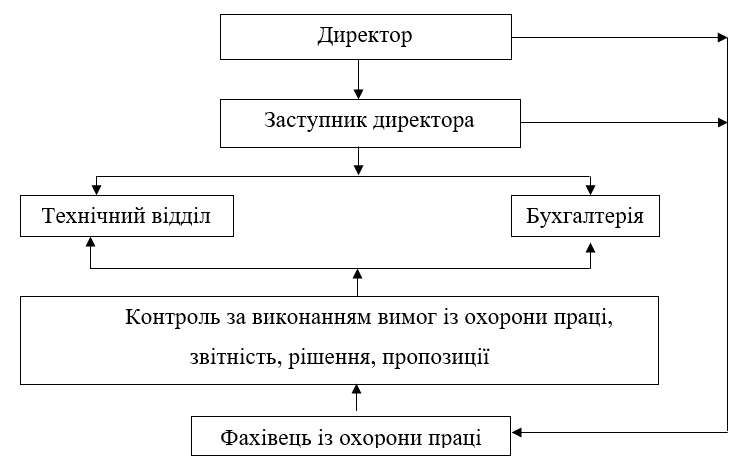
\includegraphics[width=\textwidth]{labor_structure}
	\caption{Структура \acrshort{smw}П на підприємстві}
	\label{fig:labor_structure}
\end{figure} 

Управління охороною праці здійснюється: на підприємстві у цілому --- директором підприємства безпосередньо та через заступника. 
У підрозділах та відділах --- керівниками підрозділів.
Контроль за дотриманням вимог із питань охорони праці та навколишнього середовища, підготовка звітності, рішень та пропозицій щодо покращення умов праці, виконує фахівець із охорони праці.

\subsection{Загальна характеристика приміщення та робочого місця}
Приміщення лабораторії, в якій проводяться дослідження та випробування за завданням наведені у таблиці~\ref{tab:labor_charactristics}.

\begin{table}[H]
	\caption{Загальна характеристика умов праці}
	\label{tab:labor_charactristics}
	\begin{tabular}{@{}|p{0.3\linewidth}|p{0.3\linewidth}|p{0.3\linewidth}|@{}}
	 	\hline
		Шкідливі та небезпечні фактори на робочому місці & Джерела утворювання небезпек & Примітка (данні наведені для технічного відділу) \\ \hline
		\begin{itemize}[leftmargin=*]
			\item електрична напруга вище 127В; 
			\item електромагнітні, радіаційні та теплові випромінювання; 
			\item статична електрика;
			\item іонізація повітря; 
			\item пожежна небезпека у приміщенні; 
			\item неякісне освітлення.
		\end{itemize}
		&
		Кондиціонер, 10 \acrshort{pc}, папір, світильники.
		&
		Розміри приміщення (метри):
		\begin{itemize}
			\item довжина --- 5;
			\item ширина --- 15;
			\item висота --- 3.
		\end{itemize} 
		Кількість працюючих --- 7.
		\\ \hline
	\end{tabular}
\end{table}

Приміщення має  площу 75 $\textup{м}^\textup{2}$ та об'єм 225 $\textup{м}^\textup{3}$. 
В ньому розташовано 7 (сім) робочих місць із 10 (десятьма) \acrshort{pc}. 
Таким чином площа, яка приходиться на одне робоче місце --- 10 $\textup{м}^\textup{2}$, а об'єм --- 32 $\textup{м}^\textup{3}$. 

Отже, фактичні дані  відповідають нормативним вимогам, так  як для користувачів \acrshort{pc} норма площі на одне робоче місце, обладнане комп'ютером, згідно з НПАОП 0.00-1.28-2010~\cite{Npaop2010} повинна бути більшою ніж 6 $\textup{м}^\textup{2}$ та норма об'єму --- не менш 20 $\textup{м}^\textup{3}$.

За умовами завдання це виконується повністю.

Загальні характеристики робіт, що виконуються наведені в таблиці~\ref{tab:labor_w_charactristics}.

\begin{table}[H]
	\caption{Загальна характеристика робіт, що виконуються}
	\label{tab:labor_w_charactristics}
	\begin{tabular}{@{}|p{0.3\linewidth}|p{0.3\linewidth}|p{0.3\linewidth}|@{}}
	 	\hline
		Категорія за важкістю робіт & Показники напруженості трудового процесу & Ступінь відповідальності за результат своєї діяльності \\ \hline
		І а: до 139 Вт/$\textup{м}^\textup{2}$, І б: 140-174 Вт/$\textup{м}^\textup{2}$.
		&
		Ступінь ризику для власного життя --- виключений; ступінь відповідальності за безпеку інших осіб --- виключений.
		&
		Значущість помилки --- допустимий (напруженість праці середнього ступеня); вимагає додаткових зусиль з боку керівництва; спостереження за екраном відеотерміналу (2--3 годин на зміну).
		\\ \hline
	\end{tabular}
\end{table}

\subsection{Метеорологічні параметри робочої зони}
Під час роботи з \acrshort{pc} необхідно дотримувати оптимальні метеорологічні умови. 
Оптимальні метеорологічні умови --- сполучення параметрів, які при тривалому й систематичному впливі на людину забезпечують збереження нормального функціонального й теплового стану організму без напруження реакцій терморегуляції.

За енерговитратами організму, проведення дослідницької роботи належить до категорії легких робіт <<І а>>, тому що робота проводиться сидячи і супроводжується незначними фізичними напруженнями (витрати енергії при виконанні роботи не перевищують 90--120 ккал/год).

Для даної категорії параметри мікроклімату в приміщенні повинні відповідати ДН 3.3.5-8-6.6.1-2002. 
Із урахуванням категорії роботи за енерговитратами повинні дотримуватися параметри мікроклімату, наведені в таблиці~\ref{tab:labor_climat}.

	\begin{longtabu} to \textwidth {|X[1,l]|X[1,l]|X[1,l]|X[1,l]|X[1,l]|}
  		\caption{Оптимальні параметри мікроклімату}
  		\label{tab:labor_climat} \\
		\hline
		Категорія робіт & Період року & Температура, °С &Відносна вологість, \% & Швидкість руху повітря, м/с \\
		\hline
		\endfirsthead
  		\caption*{Закінчення таблиці \thetable{}}\\
		\hline
		Категорія робіт & Період року & Температура, °С &Відносна вологість, \% & Швидкість руху повітря, м/с \\
		\hline
		\endhead

		Легка (Іа) & холодний&22--24&40--60	&не більше 0.1 \\
		\hline
		Легка (Іа) & теплий&23--25&40--60	&не більше 0.1 \\
		\hline

	\end{longtabu}

Для підтримки в приміщенні оптимального температурного режиму відповідно до вимоги СНиП 2.04.05-92 є централізоване опалювання і вентиляція. 
У теплий період року використовується кондиціювання.

\subsection{Освітлення приміщення}
Особливістю роботи за дисплеєм \acrshort{pc} є постійна й значна напруга функцій зорового аналізатора, обумовленого необхідністю розходження самосвітних об'єктів (символів, знаків і т.п.) при наявності відблисків на екрані, рядковій структурі екрана, мерехтіння зображення, недостатньою чіткістю об'єктів розходження.

Для забезпечення нормального освітлення для працівника застосовують природне, штучне та сполучене освітлення, які нормуються ДБН В.2.5-28-2006~\cite{Dbn2006} та НПАОП 0.00-1.28-2010~\cite{Npaop2010}.

По характеру зорової роботи, робота відноситься до високої точності, розряд зорової роботи III, підрозряд б. 

Раціональне освітлення приміщення сприяє кращому виконанню виробничого завдання і забезпеченню комфорту при роботі. 
Дані по нормах освітлення наведені в таблиці~\ref{tab:labor_light}.

\begin{table}[H]
	\caption{Характеристики освітленості робочого приміщення}
	\label{tab:labor_light}
	\begin{tabular}{@{}|p{0.22\linewidth}|p{0.23\linewidth}|p{0.23\linewidth}|p{0.23\linewidth}|@{}}
	 	\hline
	 	\multicolumn{3}{|l|}{Приміщення} & Відділ \\ \hline
	 	\multicolumn{3}{|l|}{\shortstack[l]{Площина нормування освітленості та КПО,\\ висота площини над рівнем підлоги}} & Г-0.8 \\ \hline
	 	\multicolumn{3}{|l|}{Розряд та підрозряд зорової роботи} & Б-1 \\ \hline
	 	\multicolumn{3}{|l|}{Вид освітлення} & Бокове \\ \hline

	 	\multirow{4}{*}{\shortstack[l]{Нормоване\\ значення}} & \multirow{2}{*}{\shortstack[l]{Штучне\\ освітлення}} & При комбінованому освітлені, лк. & 400 \\ \cline{3-4}
	 	& & При загальному освітлені, лк. & 200 \\ \cline{2-4}
	 	& \multicolumn{2}{|l|}{Природне освітлення КПО $e_n$, \%} & 1.0 \\ \cline{2-4}
	 	& \multicolumn{2}{|l|}{Суміщене освітлення КПО $e_n$, \%} & 0.6 \\ \hline
	\end{tabular}
\end{table}

Приміщення з постійним перебуванням людей повинно мати, як правило, природне освітлення. При виконанні роботи використовувалося природне одностороннє бокове й штучне освітлення. Нормативне значення КПО повинно бути не менш 1.5\% при роботі з \acrshort{pc}, тому потрібно застосовувати штучне освітлення (згідно ДБН В.2.5-28-2006~\cite{Dbn2006}).

\subsection{Шум та вібрація у робочому приміщенні}
\acrshort{pc} не створює значного шуму і вібрацій.

Джерелом шуму в робочому приміщенні є кондиціонер та лампа.
Рівень шуму в кабінеті становить 33 дБ(А). 
Взагалі рівень шуму повинен бути не більше 50 дБ(А), що є нормою для даного виду діяльності відповідно до НПАОП 0.00-1.28-2010 \cite{Npaop2010}.

Заходи по забезпеченню встановлених норм: використання спеціальних шумопоглинаючих перегородок, застосування меблів, які сприяють зменшенню шуму і вібрації, установка апаратів і приладів на спеціальні амортизуючи підкладки.

\subsection{Електробезпека у робочому приміщенні}
Для живлення устаткування (\acrshort{pc}, освітлювальні прилади) які є однофазними споживачами використовується трифазна мережа 380/220В частотою 50Гц з глухо заземленою нейтраллю.  

В правилах устрою електроустановок (згідно ПУЕ~\cite{Pue2011}) передбачені наступні заходи електробезпеки: конструктивні, схемно-конструктивні й експлуатаційні. 
Конструктивні --- це вимоги що забезпечують захист від доторкання персоналу до струмоведучих частин. 
\acrshort{pc} мають ступінь захисту ІР-44. 
Схемно-конструктивним заходом захисту є занулення електрообладнання у приміщенні.

Для користувача \acrshort{pc} важливим є дотримання правил безпеки експлуатації електрообладнання. 
Так, заборонено доторкатися до дротів та з'єднань при наявності напруги в мережі, а також самостійно проводити ремонт електрообладнання. 
Усі питання щодо ремонту налагодження та інше, можуть виконувати тільки електрики та відповідні фахівці, які мають допуск до роботи із електрообладнанням певної категорії.

\subsection{Ергономічні вимоги до робочого місця}
Робоче місце оператора \acrshort{pc} обладнується робочим столом, кріслом і підставкою для ніг. 
Висота робочого стола регулюється в межах 0.68--0.80 м., а при відсутності такої можливості має складати 0.72 м. 
Мінімальна ширина стола 0.6 м., поверхня стола не блискуча.
Робоче крісло оператора забезпечується підіймально-поворотним пристроєм з регулюванням висоти сидіння та спинки. 
Розміри підставки для ніг довжина 0.4 м., ширина не менше 0.3 м.  
На одного працюючого з урахуванням роботи з \acrshort{pc} має відводитись не менше 6 $\textup{м}^\textup{2}$ та не менше 20 $\textup{м}^\textup{3}$ об'єму приміщення згідно (НПАОП 0.00-1.28-2010~\cite{Npaop2010}).

\subsection{Пожежна безпека}
В приміщенні відсутні умови, які можуть створювати підвищену або особливо підвищену небезпеку, тому воно відноситься до класу звичайних приміщень (згідно ПУЕ-2011). 
Джерелом живлення є трифазна мережа напруги 380/220 В з глухо заземленою нейтралю, з частотою 50 Гц (згідно НПАОП 0.00-1.28-2010~\cite{Npaop2010}). 
За пожежо-вибухонебезпекою приміщення лабораторії відноситься до класу В. 
У таблиці~\ref{tab:labor_yyy} наведена характеристика робочого приміщення та категорія приміщення за вибухо-пожежної  і пожежної небезпеки. 
В таблиці~\ref{tab:labor_zzz} приведений перелік обов’язкових засобів пожежогасіння.

	\begin{longtabu} to \textwidth {|X[1,l]|X[3,l]|}
  		\caption{Оптимальні параметри мікроклімату}
  		\label{tab:labor_yyy} \\
		\hline
		Категорія приміщення & Характеристика приміщення за вибуховопожежної і пожежної небезпеки \\
		\hline
		\endfirsthead
  		\caption*{Закінчення таблиці \thetable{}}\\
		\hline
		Категорія приміщення & Характеристика приміщення за вибуховопожежної і пожежної небезпеки \\
		\hline
		\endhead

		Вибухо-пожежо-небезпечна категорія В & Звичайне, без ознак хімічного забруднення та нормальної вологості за санітарними вимогами \\
		\hline

	\end{longtabu}

{\small
	\begin{longtabu} to \textwidth {|X[2,l]|X[2,l]|X[3,l]|X[3,l]|X[4,l]|}
  		\caption{Оптимальні параметри мікроклімату}
  		\label{tab:labor_zzz} \\
		\hline
		Приміщення&Площа, м$\textup{м}^\textup{2}$&Клас зони&Первинні засоби пожежогасіння&Вогнегасний ефект \\
		\hline
		\endfirsthead
  		\caption*{Закінчення таблиці \thetable{}}\\
		\hline
		Приміщення&Площа, м$\textup{м}^\textup{2}$&Пожежнонебезпечної зони&Первинні засоби пожежогасіння&Вогнегасний ефект \\
		\hline
		\endhead

		Відділ & 50 & Клас П--ІІ & ВП-14 --- 2 одиниці, ВВК-2 --- 2 одиниці & Гасіння загорянь легкозаймистих і горючих рідин, електроустановок, що знаходяться під напругою \\
		\hline

	\end{longtabu}
}

\subsection{Охорона навколишнього природного середовища}
Закон України <<Про охорону навколишнього середовища>> визначає правові, економічні, соціальні основи охорони навколишнього середовища. 
Завдання Закону полягає в регулюванні відносин у галузі охорони праці, використанні та відновленню природних ресурсів, забезпеченні екологічної безпеки, попередженню та ліквідації наслідків негативної дії на навколишнє середовище діяльності людини, збереження природних ресурсів, генетичного фонду нації, ландшафтів й інших природних об'єктів. 

\acrshort{computer} не є джерелом яких-небудь шкідливих речовин, що забруднюють навколишнє середовище.
В ході розробки утворюються відходи у вигляді використаного паперу та канцтоварів, які збираються в спеціальний контейнер, а потім відправляються на утилізацію.

